\documentclass{standalone}

\usepackage{tikz}

\begin{document}
	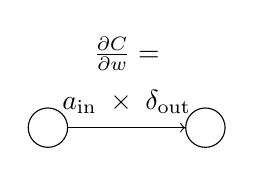
\begin{tikzpicture}[yscale = 0.75]
		\node[circle, draw, minimum size = 0.5cm] (1) at (0, 0) {};
		\node[circle, draw, minimum size = 0.5cm] (2) at (2, 0) {};
		\draw[->] (1) node[anchor = south west, inner sep = 5pt] {\(a_{\mathrm{in}}\)} to (2) node[anchor = south east, inner sep = 5pt] {\(\delta_{\mathrm{out}}\)};
		\node at (0.93, 0.43) {\(\times\)};
		\node at (1, 1.25) {\(\frac{\partial{C}}{\partial{w}} = \)};
	\end{tikzpicture}
\end{document}